\providecommand{\main}{../../..}
\providecommand{\Figures}{\main/Figures}

\documentclass[\main/main.tex]{subfiles}

\begin{document}

\chaptermark{Lempereur et al, MMTA 2020}
\chapter{\label{sec:lempereur_info}
Article 2 : Segmentations automatiques d'images 3D acquises par microscopie confocale pour la mesure de la matière blanche de cerveaux de \pz{}
}

\section{Présentation de l'article 2}
% Introduction marquage
%
Comme vu dans la \autoref{sec:bouffard}, l'emploi d'un marqueur fluorescent lipophile, par exemple l'indocarbocyanine cationique (DiI), permet de marquer les lipides se trouvant au sein d'un tissu.
%
Le marquage d'un pz{} au DiI sépare l'échantillon en deux plages d' intensités.
%
Une premier plage, très intense,
se retrouve au sein des zones très fortement lipidiques,
comme les gaines de myéline entourant certains neurones,
les jonctions serrées au sein du tube digestif ou encore le contenu du sac vitellin.
%
La seconde plage d'intensité, plus faible, correspond au marquage de l'ensemble des
enveloppes cellulaires, ce qui permet de marquer l'ensemble de l'échantillon.
%
En utilisant la différence d'intensité lumineuse induites par ces marquages,
il est possible de détecter la matière blanche se trouvant
dans le système nerveux central ainsi que l'ensemble de l'échantillon.

% Segmentation
%
Nous avons donc développé un premier algorithme visant à segmenter l'ensemble de l'échantillon,
puis un second servant à segmenter la matière blanche.
%
Au sein de ce second algorithme, une étape d'élimination de la rétine a été implémentée
afin de limiter la segmentation à la matière blanche cérébrale.
%
Ces deux algorithmes couplent des méthodes de morphologies mathématiques et de seuillages
afin d'obtenir les deux segmentations désirées en un minimum de temps.
%
Le déroulé de ces algorithmes est disponible en \autoref{sec:algo:larva} et \autoref{sec:algo:white}
pour respectivement la segmentation de l'ensemble de l'échantillon et de la larve entière.

% Pourquoi le SBDDCC?
%
Malheureusement, la diffusion de la lumière au sein du tissu, plus importante ue dans le milieu d'acquisition, induit une réduction du contraste suivant l'axe d'acquisition, déperdition plus forte dans l'échantillon.
%
Cette déperdition, qui suit la loi de Beer-Lambert, induit une imprécision de la détection de la matière blanche dans les zones profondes du cerveau.
%
Par exemple, dans le cas d'une acquisition dorsale,
cette déperdition peut induire une sous-segmentation de l'hypothalamus.
%
Afin de compenser cette déperdition, nous avons développé un algorithme de compensation
utilisant la segmentation de l'échantillon entier, et que nous avons nommé \sbddcc{} (SBDDCC).

% Fonctionnement du SBDDCC
%
Pour initier le SBDDCC,
on commence par calculer une carte de la profondeur au sein de l'échantillon.
%
Cette carte consiste en une somme cumulative de la segmentation de l'échantillon entier
suivant l'axe d'acquisition.
%
Cette carte permet le calcul des valeurs de gris médianes pour chaque couche.
%
On normalise ensuite la valeur des médians des couches profondes pour qu'elle vaillent la même valeur que le médian maximal.
%
Cet algorithme de correction,
qui compense une décroissance exponentielle comme prédit par la loi de Beer-Lambert,
a l'intérêt de ne nécessiter qu'une seule acquisition, contrairement aux méthodes de tomographie.
%
De plus, il permet de réduire le temps de calcul contrairement à des méthodes plus complexes.
%
En revanche, la réduction de cette correction à la segmentation de l'échantillon entier permet
d'améliorer l'application de cette méthode de calcul en tenant compte de la forme de
l'échantillon.

% Condensé des résultats
En résumé, les résultats principaux de la publication au sein de
\emph{Mathematical Morphology - Theory and Application} sont les suivants:
\begin{itemize}
    %larve entière
    \item 
    Le marquage d'un \pz{} au DiI permet la mise en place
    d'un algorithme de segmentation de l'intégralité de l'échantillon (voir \autoref{fig:lempereur_info:whole}).
    
    \item
    Cette algorithme couple des procédures de seuillages et de morphologies mathématiques 
    afin d'initier le calcul de \watersheds.
    
    \item
    L'algorithme de segmentation de l'intégralité de l'échantillon fournit
    rapidement et de manière robuste un résultat précis.
    
    %sbddcc
    \item
    Malgré l'emploi d'une clarification optique,
    Un phénomène de diffusion suivant la loi de Beer-Lambert peut apparaître au sein de l'échantillon.
    
    \item
    En ce basant sur la segmentation de la larve entière,
    un algorithme de compensation de l'atténuation lumineuse a été développé, nommé \sbddcc 
    (voir \autoref{fig:lempereur_info:correction}).
    
    \item
    Le SBDDCC commence par mesurer la profondeur au sein de l'échantillon
    
    \item
    Le SBDDCC calcule ensuite le médian des valeurs de gris pour chaque coupe.
    
    \item
    Le SBDDCC égalise le médian des valeurs de gris des couches profondes au médian maximal.
    
    \item
    La valeur médiane des niveaux de gris pour chaque profondeur suivant une décroissance exponentielle,
    cet algorithme permet de compenser la loi de Beer-Lambert.
    
    \item
    Cet algorithme permet d'effectuer peu de calcul, et permet de simplifier les acquisitions.
    
    \item
    L'algorithme de compensation permet d'améliorer significativement 
    la qualité du recalage de deux acquisitions du même échantillon.
    
    \item
    De plus, cet algorithme de compensation permet à un opérateur spécialisé
    d'améliorer la précision de ses segmentations manuelles.
    
    %Matière blanche cérébrale
    \item
    En utilisant une seconde fois le marqueur lipophile, un algorithme de segmentation de la matière blanche cérébrale a été mis au point en couplant des méthodes de morphologies mathématiques à des seuillages (Voir \autoref{fig:lempereur_info:white}).
    
    \item
    Cet algorithme de segmentation de la matière blanche utilise
    l'algorithme de compensation afin d'améliorer sa précision.
    
    \item
    Afin de limiter la segmentation de la matière blanche au cerveau,
    un algorithme de détection des rétines a été développé.
    
    \item
    L'algorithme de segmentation de la matière blanche fournit rapidement un résultat précis. 
    
\end{itemize}

%
Enfin, l'algorithme de segmentation de la matière blanche cérébrale a servi de base au
développement de la segmentation de la matière grise présentée en \autoref{sec:HuC},
et le SBDDCC a servi de base pour le développement d'un algorithme de compensation
d'un défaut de marquage \ihc{} présenté en \autoref{sec:sblc}.

\begin{figure}[!h]
    \centering
    \begin{subfigure}[b]{0.45\textwidth}
       \caption{
            \label{fig:lempereur_info:brut}
            Données brutes obtenues par marquage liphohile
            }
       \centering 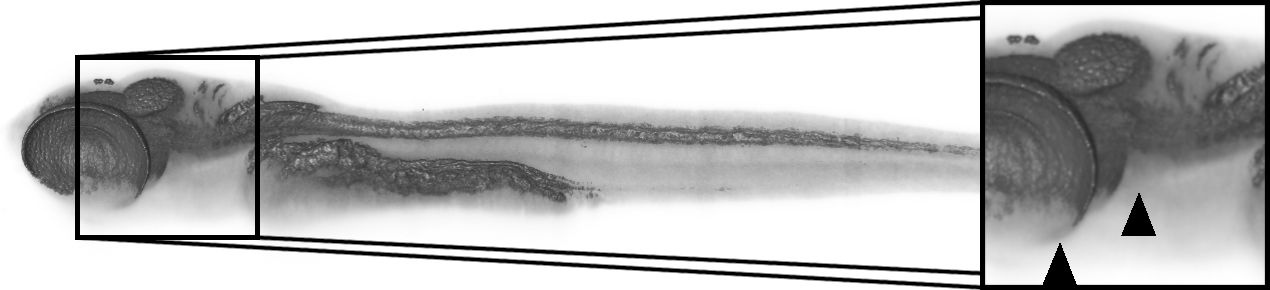
\includegraphics[width=\textwidth]{\Figures/Segmentations/original.png}
    \end{subfigure}
    \begin{subfigure}[b]{0.45\textwidth}
       \caption{
        \label{fig:lempereur_info:whole}
        Segmentation de l'échantillon
        }
       \centering 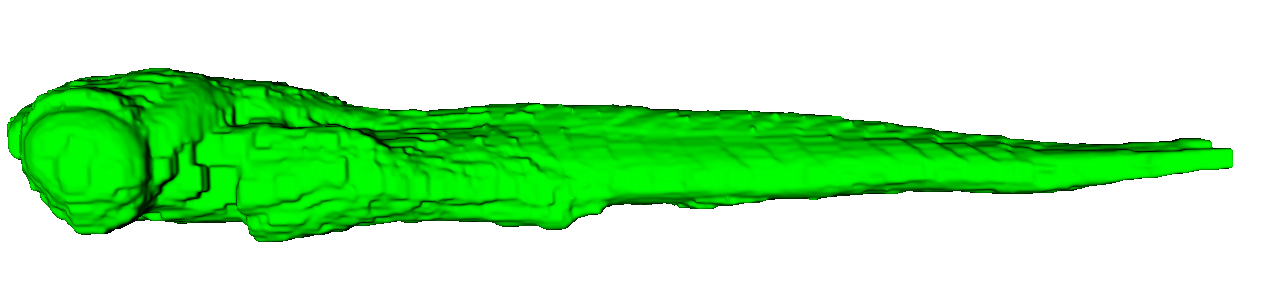
\includegraphics[width=\textwidth]{\Figures/Segmentations/whole.png}
    \end{subfigure}
    \begin{subfigure}[b]{0.45\textwidth}
       \caption{
           \label{fig:lempereur_info:correction}
           Données après SBDDCC
        }
       \centering 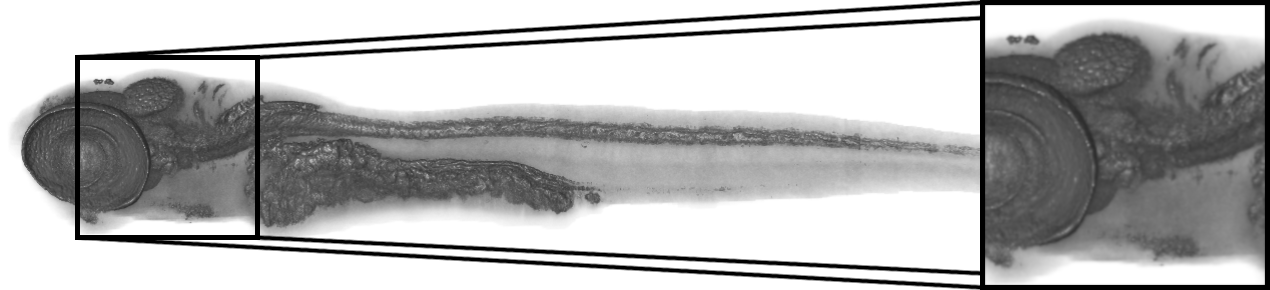
\includegraphics[width=\textwidth]{\Figures/Segmentations/contrast_corrected.png}
    \end{subfigure}
    \begin{subfigure}[b]{0.45\textwidth}
       \caption{
           \label{fig:lempereur_info:white}
            Segmentation de la matière blanche superposé aux données après SBDDCC
            }
       \centering 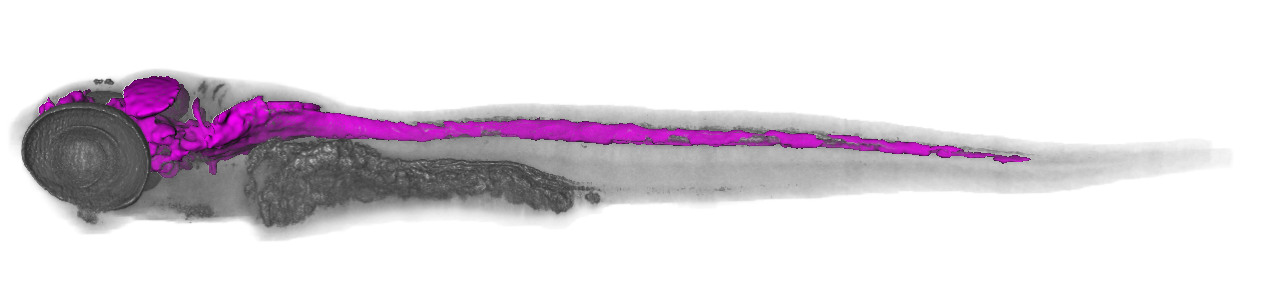
\includegraphics[width=\textwidth]{\Figures/Segmentations/white_on_corrected.png}
    \end{subfigure}
    \caption{
        \label{fig:lempereur_info}
        Représentation 3D des résultats de l'application des algorithmes sur des alevins de \pz{}.
        \newline
        (a) On aperçoit le signal faible permettant de segmenter la larve entière, ainsi que de fort marquage dans diverses régions dont la matière blanche du cerveau. L'encart met en évidence le défaut de pénétration de la lumière dans les régions profondes. Les têtes de flèche indique en particulier  perte de signal dans la partie ventrale de la rétine et dans l'hypothalamus.
        (b) L'algorithme de segmentation de l'alevin entier permet d'obtenir une segmentation précise de l'échantillon malgré la présence de la déperdition lumineuse au sein de l'échantillon.
        (c)
        En revanche, il est nécessaire de compenser cette déperdition lumineuse pour obtenir une segmentation correcte de la matière blanche. L'algorithme nommé SBDDCC nécessite la segmentation  montré en b de façon à connaître la forme de l'échantillon et ainsi mesurer la quantité de tissu traversé.
        Cet algorithme permet de compenser efficacement les défauts de pénétration de la lumière, comme on peut le voir dans l'encart (Têtes de flèche).
        (d) L'application du SBDDCC permet d'effectuer une segmentation précise de la matière blanche. L'algorithme développé est en mesure de supprimer les régions fortement marquées mais extérieur au système nerveux central, comme les rétines ou le sac vitellin.
        \newline
        Les segmentations sont représentées par des rendus surfaciques quand les données en valeurs de gris sont représentées par des rendus volumiques.
    }
    
\end{figure}

\sectionmark{Article 2 publié dans MMTA 2019}
\section{Article 2 publié dans Mathematical Morphology\hyp{}Theory and Applications}

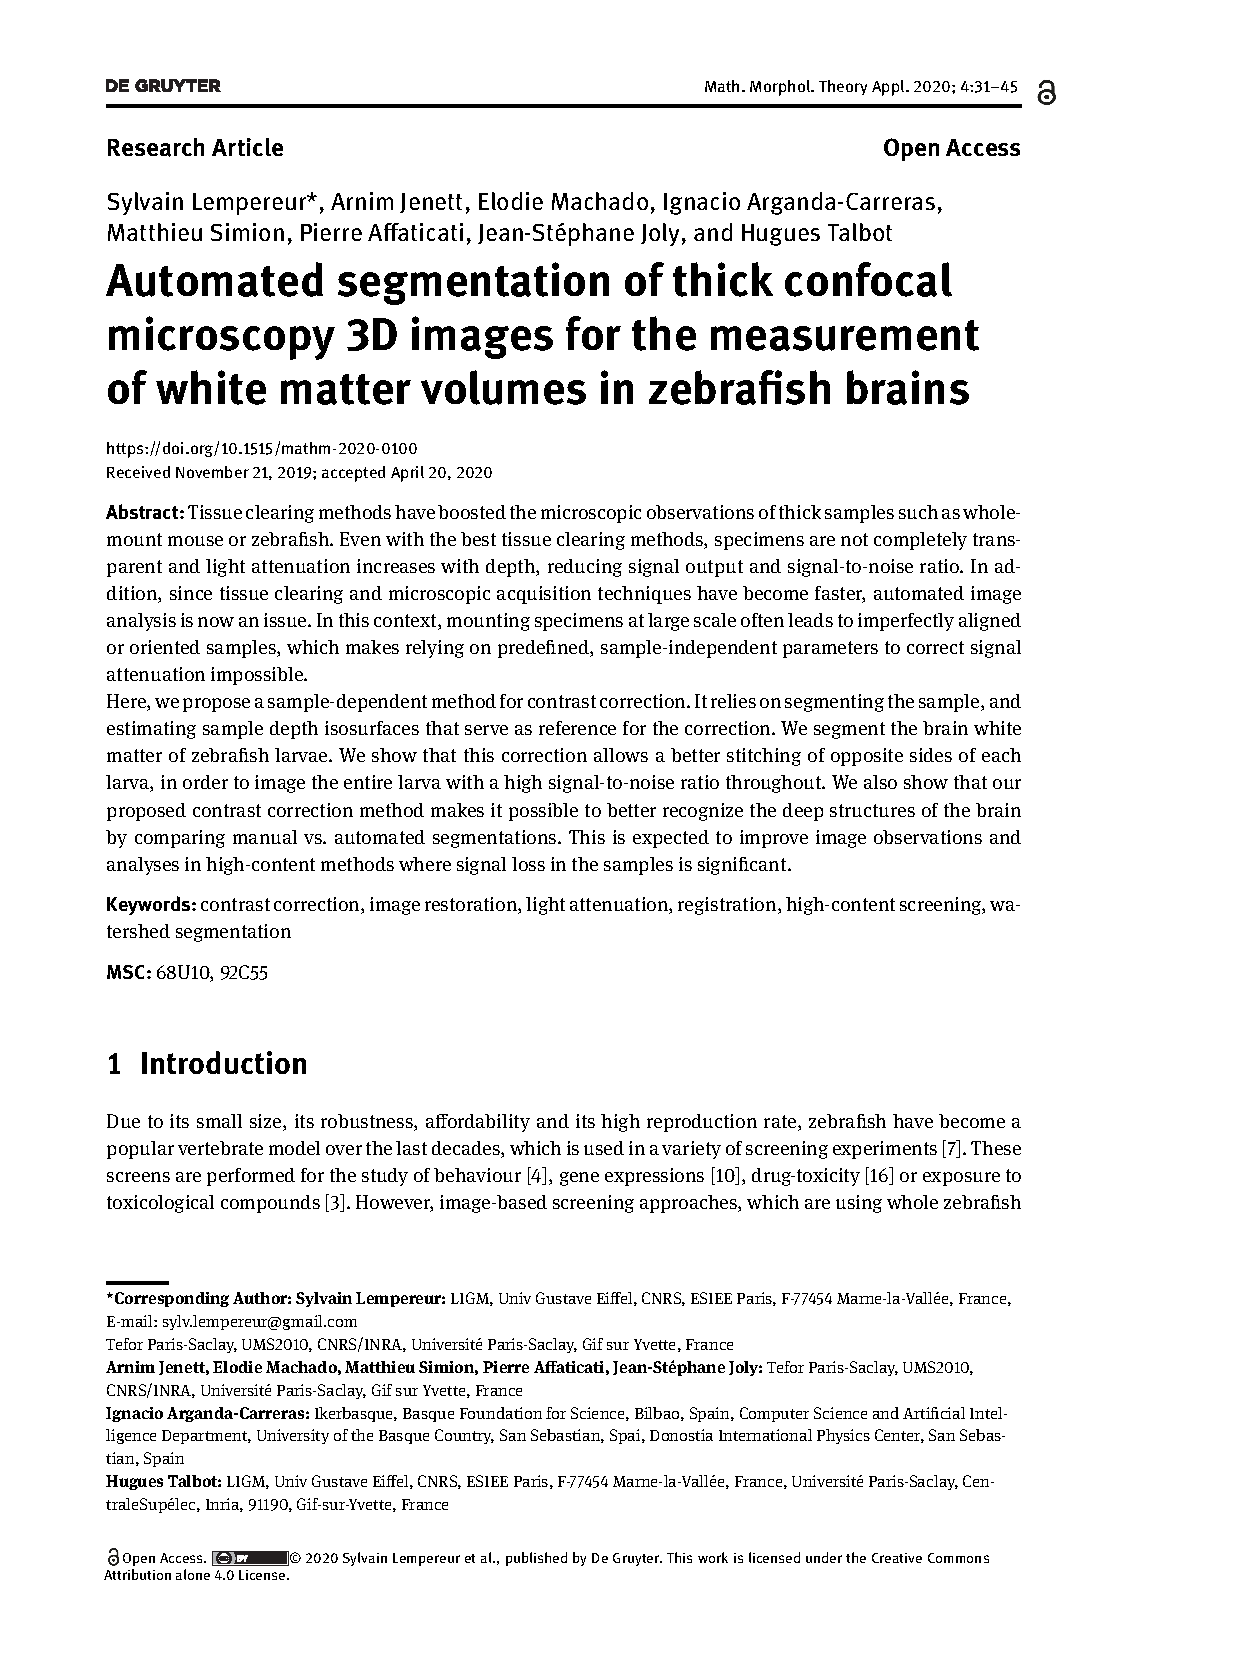
\includepdf[pages=-]{./mmta2020.pdf}

\end{document}
